\begin{frame}{Installing JupyterLab on MS Windows 10 (1/3)}
\begin{columns}
\begin{column}{0.6\textwidth}
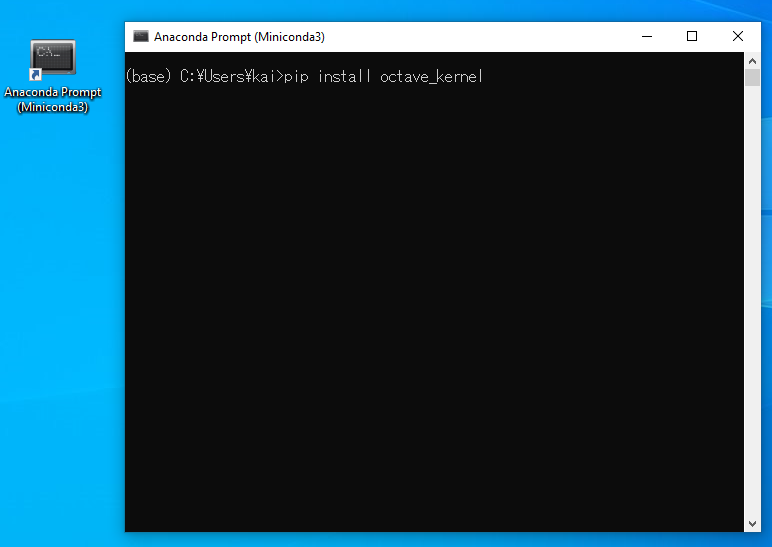
\includegraphics[width=\textwidth]{res/ms_windows/win_miniconda.png}
\end{column}
\begin{column}{0.4\textwidth}
\begin{itemize}
\itemsep2em
\item
Get Miniconda for Python \textbf{\color{DarkBlue}3.7} from
{\color{DarkBlue}\url{https://docs.conda.io/en/latest/miniconda.html}}

\item
Start "Anaconda Prompt":

\texttt{pip install jupyterlab}

\texttt{pip install sympy}

\texttt{pip install octave\_kernel}
\end{itemize}
\end{column}
\end{columns}
\end{frame}

\begin{frame}{Installing JupyterLab on MS Windows 10 (2/3)}
\begin{center}
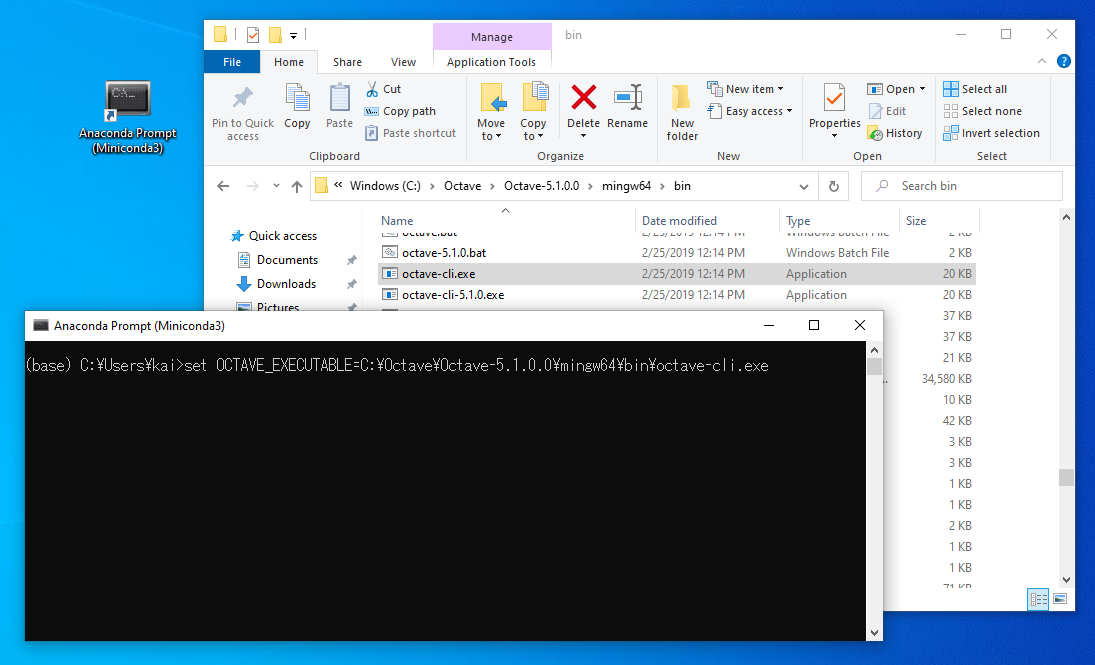
\includegraphics[width=0.7\textwidth]{res/ms_windows/win_miniconda_octave_path.png}

{\small Run:
\texttt{set OCTAVE\_EXECUTABLE=C:\textbackslash Octave\textbackslash
Octave-5.1.0.0\textbackslash mingw64\textbackslash bin\textbackslash
octave-cli.exe}}
\end{center}
\end{frame}

\begin{frame}{Installing JupyterLab on MS Windows 10 (3/3)}
\begin{columns}
\begin{column}{0.7\textwidth}
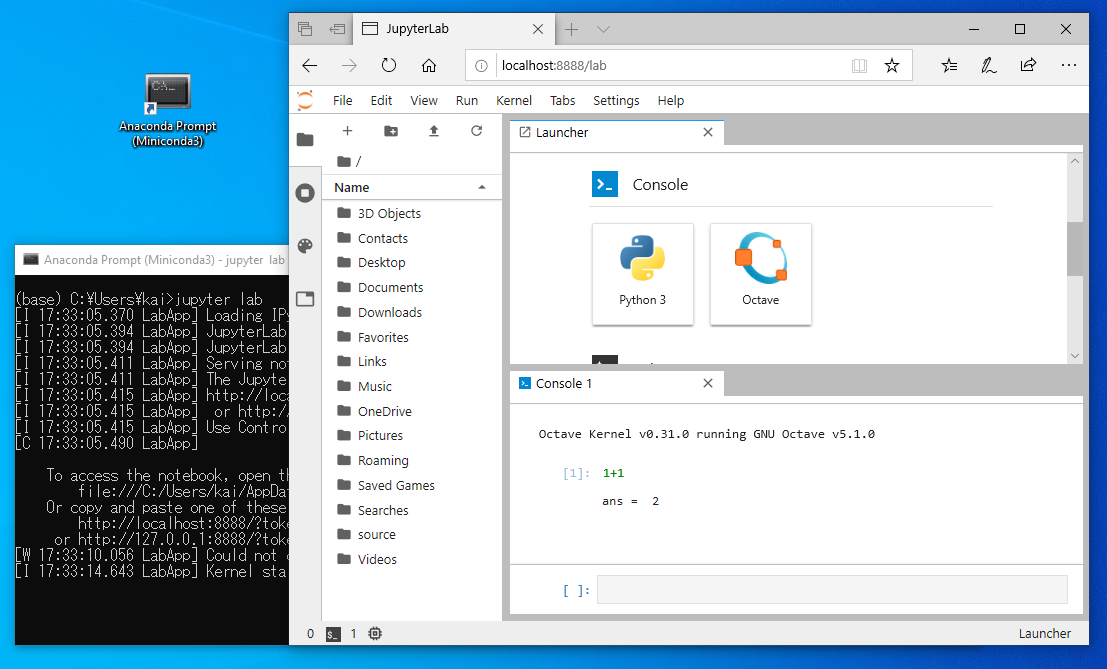
\includegraphics[width=\textwidth]{res/ms_windows/win_miniconda_jupyterlab.png}
\end{column}
\begin{column}{0.3\textwidth}
\begin{itemize}
\itemsep4em
\item
Run:

\texttt{jupyter lab}

\item
The default browser will open with the locally started JupyterLab server.
\end{itemize}
\end{column}
\end{columns}
\end{frame}